\documentclass{article}


\usepackage[T1]{fontenc} % encodage
\renewcommand{\familydefault}{\sfdefault} % police en sans-serif

\usepackage[french]{babel} % langue
\frenchsetup{SmallCapsFigTabCaptions=false}

\usepackage[hidelinks]{hyperref} % liens cliquable dans la table des matières

\usepackage{graphicx} % images
\usepackage{caption}

\usepackage[a4paper, left=20mm, top=20mm]{geometry} % dimensions de la page

\usepackage{minted} % intégration code
\usemintedstyle{emacs}

\title{Projet - IA pour le jeu d'Othello
    \thanks{\href{https://jj.up8.site/AA/ProjetsAA.pdf}{Sujet 35}}}
\author{\href{mailto:anri.kennel@etud.univ-paris8.fr}{Anri Kennel}
    \thanks{Numéro d'étudiant : 20010664}\, (L3-A)
    \\Algorithmique avancée $\cdot$ Université Paris 8}
\date{Année universitaire 2022-2023}

\begin{document}
\maketitle
\tableofcontents
\clearpage

\section{Projet}
Ce projet présente une implémentation d'un jeu d’Othello ainsi que deux
intelligences artificielles jouant; l'une selon un algorithme minimax et l'autre
via élagage alpha-bêta. Il y a aussi une comparaison d'efficacité des IA à
différentes profondeurs de jeu.

\section{Implémentation}
\subsection{Othello}
\subsubsection{Règles du jeu}
L'Othello est un jeu qui se joue sur un plateau de 8x8 où deux couleurs, les noirs
et les blancs s'affrontent. Les noirs commencent la partie. Quand aucun joueur
ne peut jouer, la partie s'arrête.

Au début d'une partie le plateau ressemble à la \autoref{fig:init}.

\begin{figure}[h]
    \centering
    \includegraphics[width=0.35\textwidth]{imgs/othello_init.png}
    \caption{Début d'une partie}
    \label{fig:init}
\end{figure}

\subsubsection{Exemple d'une partie}
Chaque joueur doit poser un pion de sa couleur sur une case vide de l’othellier,
il faut prendre en sandwich les pions ennemis, peu importe la direction. Une fois
posé, les pions prient en sandwich sont récupérés par le joueur qui vient de jouer.

Dans la configuration du début, les cases pouvant être joué par les noirs sont
indiqués en rouge dans la \autoref{fig:prem}.

\begin{figure}[h]
    \centering
    \includegraphics[width=0.35\textwidth]{imgs/othello_premiercoup.png}
    \caption{Possibilités au premier coup}
    \label{fig:prem}
\end{figure}

Mon implémentation du jeu indique au joueur les coups possibles (c'est-à-dire les
cases rouges). Le joueur doit indiquer les coordonnées où il veut poser son jeton
et les changements se font automatiquement. Chaque joueur joue chacun son tour et
passe son tour si aucun coup lui est possible. La partie s'arrête si le plateau
est plein ou si aucun joueur ne peut jouer, cf. \autoref{fig:human}. Les jetons
blancs sont notés \texttt{B} et les jetons noirs \texttt{N}.

\begin{figure}[h]
    \centering
    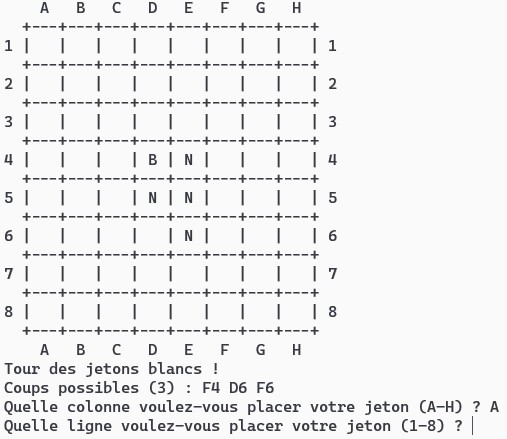
\includegraphics[width=0.35\textwidth]{imgs/othello_impl_player.jpg}
    \caption{Demande au joueur de jouer}
    \label{fig:human}
\end{figure}

Si un coup illégale est joué, le jeu refuse le coup et demande au joueur de
choisir un autre coup.

\subsubsection{Problèmes rencontrés}
Mon enjeu numéro 1 était d'éviter tout problème de mémoire. Pour cela dans le
\texttt{Makefile} il y a un label \texttt{dev} qui permet d'ajouter plein de flags
pour \texttt{gcc}, notamment \texttt{fanalyzer} et \texttt{fsanitize=undefined} qui
permettent de trouver plein de problèmes relatifs à la mémoire. Aussi j'ai utilisé
\texttt{Valgrind} (avec les flags \texttt{g} et \texttt{Og} pour \texttt{gcc} et
les flags \texttt{leak-check=full}, \texttt{show-leak-kinds=all},
\texttt{track-origins=yes} et \texttt{s} pour \texttt{Valgrind}) me permettant
d'avoir un maximum d'avertissements et d'informations me permettant de débugger
tous les problèmes.
\\\\
Aussi, je voulais rendre mon code modulable, pour tester plus facilement. Ainsi
la taille du plateau est complètement modulable, aussi les couleurs des joueurs
(cf. \autoref{cod:plateau}).

\begin{figure}[h]
    \centering
    \begin{minipage}{0.8\textwidth}
        \begin{minted}[autogobble,linenos]{c}
            /* Une case est soit vide, soit occupé par un des joueurs, noir ou blanc */
            enum CASE { VIDE = ' ', BLANC = 'B', NOIR = 'N' };
        \end{minted}

        \begin{minted}[autogobble,linenos,firstnumber=last]{c}
            /* Propriété globale du jeu */
            enum PLATEAU { LONGEUR = 8, LARGEUR = 8 };
        \end{minted}
    \end{minipage}
    \caption{Début de \texttt{jeu.h}}
    \label{cod:plateau}
\end{figure}

Enfin, sachant qu'il faut aussi implémenter des IAs, j'ai fait en sorte que le jeu
du joueur humain ne soit pas complètement lié au fonctionnement du jeu. Le projet
est donc séparé en plusieurs fichiers/fonctions (cf. \autoref{tree:project}).
\\\\
Grâce à ça, les fonctions relatives au jeu sont indifférentes par rapport à quelle
fonction "joueur" est appelée. Autrement dit, tout ce qui est relatif à un joueur
humain est dans \texttt{humain.h}. Le fichier \texttt{joueur.h} ne contient rien
spécifique à un joueur humain.

\begin{figure}[ht]
    \centering
    \begin{minipage}{0.15\textwidth}
        \begin{minted}[autogobble,frame=lines,rulecolor=gray]{mcf}
            - includes
            |-- humain.h
            |-- jeu.h
            |-- joueur.h
            |-- liste.h
            |-- plateau.h
            \-- utils.h
            - src
            |-- humain.c
            |-- jeu.c
            |-- joueur.c
            |-- liste.c
            |-- main.c
            |-- plateau.c
            \-- utils.c
        \end{minted}
    \end{minipage}
    \caption{Arborescence du projet sans l'implémentation des IA et tests}
    \label{tree:project}
\end{figure}

\newpage
\subsection[Minimax]{Algorithme minimax}
\subsubsection{Algorithme}
L'idée de l'algorithme minimax est de calculer tous les coups possibles pour
chaque coup possible et d'aller le plus loin possible dans les "et si" pour faire
le coup qui nous rapportera le plus de points dans le futur.

Le problème de cet algorithme c'est qu'il est difficilement réalisable. En mémoire,
on doit copier le plateau plusieurs fois (pour chaque "et si"). La complexité est
de $\Theta(c^{n})$ avec $c$ les coups légaux et $n$ la profondeur de jeu, donc
lorsque l'on utilise cet algorithme on doit garder notre profondeur de test
relativement basse.

Aussi, l'algorithme est dépendant d'une fonction d'évaluation, c'est elle qui
décide si le coup est bien ou non, plus elle est précise plus le coup décidé sera
meilleur.

\subsubsection{Exemple d'utilisation}
L'utilisation de l'algorithme est simple. Il suffit d'appeler une seule fonction
et elle jouera un coup (cf. \autoref{cod:minimax_def}).
\begin{figure}[h]
    \centering
    \begin{minipage}{0.8\textwidth}
        \begin{minted}[autogobble,linenos]{c}
            /* Joue le tour d'après l'algorithme minimax */
            void action_joueur_minimax(Jeu *jeu, const int couleur, const int profondeur);
        \end{minted}

        \begin{minted}[autogobble,linenos,firstnumber=last]{c}
            /* Auxiliaire : Décide d'une case à jouer via l'algorithme minimax */
            void _action_joueur_minimax(Jeu *jeu, int profondeur, const int couleur,
                                        const int gagnant, int *ligne, int *colonne,
                                        int *score);
        \end{minted}
    \end{minipage}
    \caption{Déclaration de minimax, dans \texttt{minimax.h}}
    \label{cod:minimax_def}
\end{figure}

Pour l'utiliser, il faut l'appeler dans la fonction qui s'occupe du déroulement
du jeu (cf. \autoref{cod:minimax_play}).

\begin{figure}[ht]
    \centering
    \begin{minipage}{0.8\textwidth}
        \begin{minted}[autogobble,linenos]{c}
            while (!partie_finie(jeu)) {
                Coups *possibilites =
                    action_possible_joueur(jeu->plateau, tour->couleur);
                if (possibilites->taille_liste > 0) {
                    // Si le joueur peut jouer
                    if (tour->couleur == NOIR) {
                        // Tour du joueur minimax
                        action_joueur_minimax(jeu, tour->couleur, profondeur);
                    } else {
                        // Tour du joueur humain
                        action_joueur_humain(jeu, tour->couleur, profondeur);
                    }
                }

                // On passe la main à l'autre joueur
                tour = jeu->j1->couleur == tour->couleur ? jeu->j2 : jeu->j1;
            }
        \end{minted}
    \end{minipage}
    \caption{Extrait simplifié de \texttt{jeu.c}, avec minimax jouant les noirs et un humain les blancs}
    \label{cod:minimax_play}
\end{figure}

\newpage
\subsubsection{Problèmes rencontrés}
Le plus dur était l'implémentation en elle-même et de pas s'emmêler entre les copies
de plateau. La fonction \texttt{action\_joueur\_minimax} appelle une fonction auxiliaire
\texttt{\_action\_joueur\_minimax} (cf. \autoref{cod:minimax_def}) qui fait implémente directement minimax. Elle se passe
en paramètre récursivement :
\begin{itemize}
    \item la ligne choisie
    \item la colonne choisie
    \item le meilleur score
    \item la profondeur actuellement évaluée
    \item la couleur du joueur (soit MIN, soit MAX)
\end{itemize}

\subsection[Alpha-Bêta]{Élagage alpha-bêta}
\subsubsection{Algorithme}
Les coupures $\alpha - \beta$ permettent de réduire la taille en mémoire de minimax
en ne calculant pas certains scénarios en retirant ceux inutiles basé sur
les calculs précédents.

\subsubsection{Exemple d'utilisation}
L'utilisation est identique à celle de Minimax (cf. \autoref{cod:alphabeta_def}).
\begin{figure}[h]
    \centering
    \begin{minipage}{0.8\textwidth}
        \begin{minted}[autogobble,linenos]{c}
            /* Joue le tour d'après l'algorithme alpha-beta */
            void action_joueur_alphabeta(Jeu *jeu, const int couleur);
        \end{minted}

        \begin{minted}[autogobble,linenos,firstnumber=last]{c}
            /* Auxiliaire : Décide d'une case à jouer via l'algorithme alpha-beta */
            void _action_joueur_alphabeta(Jeu *jeu, int profondeur, int couleur,
                                        const int gagnant, int *ligne, int *colonne,
                                        int *score, const int note, const int qui);
                                                        // qui => couleur associée
        \end{minted}
    \end{minipage}
    \caption{Déclaration d'alphabeta, dans \texttt{alphabeta.h}}
    \label{cod:alphabeta_def}
\end{figure}

\subsubsection{Problèmes rencontrés}
Pour l'implémentation je me passe en argument, en plus de ceux de minimax, le
meilleur score et sa couleur associée.

L'avantage avec cet algorithme est qu'il ressemble beaucoup à minimax vu que c'est
une amélioration de ce dernier, alors j'ai pu réutiliser le même code. En revanche
l'élagage était compliqué à placer dans le code.

Je fais l'élagage en passant des possibilités pour alpha (cf. \autoref{cod:elagage_alpha}),
même technique pour bêta (cf. \autoref{cod:elagage_beta}).

\begin{figure}[h]
    \centering
    \begin{minipage}{0.8\textwidth}
        \begin{minted}[autogobble,linenos]{c}
            while (i->suivant) {
                if (i->suivant->suivant) {
                    i = i->suivant;
                } else {
                    break;
                }
            }
            *score = INT_MAX;
        \end{minted}
        \dots\, et \dots
        \begin{minted}[autogobble,linenos,firstnumber=last]{c}
            if (*score == INT_MAX) {
                while (i->suivant) {
                    if (i->suivant->suivant) {
                        i = i->suivant;
                    } else {
                        break;
                    }
                }
            }
        \end{minted}
    \end{minipage}
    \caption{Élagage $\alpha$, dans \texttt{alphabeta.h}}
    \label{cod:elagage_alpha}
\end{figure}

\begin{figure}[h]
    \centering
    \begin{minipage}{0.8\textwidth}
        \begin{minted}[autogobble,linenos]{c}
            while (i->suivant) {
                if (i->suivant->suivant) {
                    i = i->suivant;
                } else {
                    break;
                }
            }
            *score = INT_MIN;
        \end{minted}
        \dots\, et \dots
        \begin{minted}[autogobble,linenos,firstnumber=last]{c}
            if (*score == INT_MIN) {
                while (i->suivant) {
                    if (i->suivant->suivant) {
                        i = i->suivant;
                    } else {
                        break;
                    }
                }
            }
        \end{minted}
    \end{minipage}
    \caption{Élagage $\beta$, dans \texttt{alphabeta.h}}
    \label{cod:elagage_beta}
\end{figure}

\section{Comparaison d'efficacité}
Le fichier \texttt{text.h} déclare une série de fonctions qui permet de tester
minimax et alpha-bêta.
Je teste 2 facette des IA, la rapidité d'exécution et le taux de victoire des
IA (cf. \autoref{txt:tests_res}).
\label{sec:comp_eff}

La partie test de rapidité permet de montrer que l'implémentation d'alpha-bêta
fonctionne car a profondeur égale, alpha-bêta est beaucoup plus rapide que
minimax. Je n'ai d'ailleurs pas testé minimax sur d'aussi grandes profondeurs
qu'alpha-bêta car cela prenait trop de temps. Le temps total des tests dure
environ 4 minutes sur ma machine.

Cette partie montre aussi qu'il n'y a pas grande différence en temps entre
minimax et alpha-bêta pour une profondeur inférieur ou égal à 4.

La partie sur le taux de victoire permet de montrer qu'à profondeur égale,
alpha-bêta et minimax ne se démarquent pas, et que c'est bien la différence de
profondeur qui donne l'avantage.

En effet, là où minimax prend beaucoup de temps à partir d'une profondeur de 5,
alpha-bêta peut aller jusqu'à une profondeur de 8.

À noter que lors des tests, je fais jouer l'algorithme contre lui-même donc en
réalité, l'algorithme prend 2x moins de temps que le temps indiqué, vu qu'il joue
pour les 2 joueurs. En revanche ça ne veut pas dire que l'on peut doubler la
profondeur car l'augmentation n'est pas linéaire.

\section{Conclusion}
Le problème de mon implémentation est la fonction d'évaluation qui regarde juste
le nombre de points gagnés/perdus. En ne prenant pas en compte par exemple si le
pion placé est sur un coin ou non (le coin étant une position avantageuse).

Enfin, je ne teste pas la quantité de mémoire utilisés par les algorithmes.

\newpage
\appendix
\section*{Appendix}
\listoffigures

\vspace{1cm}
\begin{figure}[h]
    \centering
    \begin{minipage}{1\textwidth}
        \begin{minted}[autogobble,linenos,fontsize=\footnotesize]{text}
            $ ./othello -t
        \end{minted}
        \begin{minted}[autogobble,linenos,fontsize=\footnotesize,firstnumber=last]{text}
            Lancement des tests, on va jusqu'à une profondeur de 8 avec une moyenne de 5 répétitions.
            On fait jouer alpha-bêta contre lui-même puis minimax contre lui-même.
            Profondeur de 1 (moyenne de 5 tests) ->  alpha-bêta = 0.001742s | minimax = 0.001829s    | différence (m - a) = 0.000087s
            Profondeur de 2 (moyenne de 5 tests) ->  alpha-bêta = 0.007442s | minimax = 0.011332s    | différence (m - a) = 0.003890s       avec le précédent = 0.003803s
            Profondeur de 3 (moyenne de 5 tests) ->  alpha-bêta = 0.029347s | minimax = 0.073701s    | différence (m - a) = 0.044354s       avec le précédent = 0.040464s
            Profondeur de 4 (moyenne de 5 tests) ->  alpha-bêta = 0.117613s | minimax = 0.344193s    | différence (m - a) = 0.226580s       avec le précédent = 0.182226s
            Profondeur de 5 (moyenne de 5 tests) ->  alpha-bêta = 0.524146s | minimax = 4.843884s    | différence (m - a) = 4.319738s       avec le précédent = 4.093158s
            Profondeur de 6 (moyenne de 5 tests) ->  alpha-bêta = 1.507593s
            Profondeur de 7 (moyenne de 5 tests) ->  alpha-bêta = 23.077325s
            Profondeur de 8 (moyenne de 5 tests) ->  alpha-bêta = 13.677932s
        \end{minted}
        \begin{minted}[autogobble,linenos,fontsize=\footnotesize,firstnumber=last]{text}
            Alpha-bêta      a gagné (profondeur minimax = 1 vs 1 = profondeur alphabêta) en tant que blanc
            Minimax         a gagné (profondeur minimax = 2 vs 1 = profondeur alphabêta) en tant que noir
            Minimax         a gagné (profondeur minimax = 3 vs 1 = profondeur alphabêta) en tant que noir
            Minimax         a gagné (profondeur minimax = 4 vs 1 = profondeur alphabêta) en tant que noir
            Alpha-bêta      a gagné (profondeur minimax = 1 vs 2 = profondeur alphabêta) en tant que noir
            Minimax         a gagné (profondeur minimax = 2 vs 2 = profondeur alphabêta) en tant que blanc
            Alpha-bêta      a gagné (profondeur minimax = 3 vs 2 = profondeur alphabêta) en tant que noir
            Minimax         a gagné (profondeur minimax = 4 vs 2 = profondeur alphabêta) en tant que blanc
            Alpha-bêta      a gagné (profondeur minimax = 1 vs 3 = profondeur alphabêta) en tant que blanc
            Minimax         a gagné (profondeur minimax = 2 vs 3 = profondeur alphabêta) en tant que noir
            Alpha-bêta      a gagné (profondeur minimax = 3 vs 3 = profondeur alphabêta) en tant que blanc
            Minimax         a gagné (profondeur minimax = 4 vs 3 = profondeur alphabêta) en tant que noir
            Alpha-bêta      a gagné (profondeur minimax = 1 vs 4 = profondeur alphabêta) en tant que noir
            Alpha-bêta      a gagné (profondeur minimax = 2 vs 4 = profondeur alphabêta) en tant que noir
            Alpha-bêta      a gagné (profondeur minimax = 3 vs 4 = profondeur alphabêta) en tant que noir
            Alpha-bêta      a gagné (profondeur minimax = 4 vs 4 = profondeur alphabêta) en tant que noir
            Minimax         a gagné (profondeur minimax = 1 vs 5 = profondeur alphabêta) en tant que noir
            Alpha-bêta      a gagné (profondeur minimax = 2 vs 5 = profondeur alphabêta) en tant que blanc
            Alpha-bêta      a gagné (profondeur minimax = 3 vs 5 = profondeur alphabêta) en tant que blanc
            Minimax         a gagné (profondeur minimax = 4 vs 5 = profondeur alphabêta) en tant que noir
            Alpha-bêta      a gagné (profondeur minimax = 1 vs 6 = profondeur alphabêta) en tant que noir
            Alpha-bêta      a gagné (profondeur minimax = 2 vs 6 = profondeur alphabêta) en tant que noir
            Alpha-bêta      a gagné (profondeur minimax = 3 vs 6 = profondeur alphabêta) en tant que noir
            Alpha-bêta      a gagné (profondeur minimax = 4 vs 6 = profondeur alphabêta) en tant que noir
            Nombre totale de parties : 24.
            Alpha-bêta a gagné      15 fois.
            Minimax a gagné         9 fois.
            Il y a eu               0 égalités.
        \end{minted}
        \begin{minted}[autogobble,linenos,fontsize=\footnotesize,firstnumber=last]{text}
            ________________________________________________________
            Executed in  234.85 secs    fish           external
               usr time  234.83 secs   62.00 micros  234.83 secs
               sys time    0.02 secs  105.00 micros    0.02 secs
        \end{minted}
    \end{minipage}
    \caption{Résultat des tests, sous commande \texttt{time} (cf. \autoref{sec:comp_eff})}
    \label{txt:tests_res}
\end{figure}

\end{document}
